\documentclass[t]{beamer}

\usepackage[utf8]{inputenc}
\usepackage[T1]{fontenc}
\usepackage{helvet}
\usepackage[english]{babel}

\usetheme{LUH}


% format numbers
\usepackage{siunitx}
%https://tex.cloud.uni-hannover.de/project/6677e7bc8f12321099572893
\sisetup{
  locale=US,
  group-digits = integer,
  round-mode = places,
  round-precision = 3,
  round-pad = false,
  mode = match % the numbers are printed in text or math mode matching their surrounding
}
% better itemize and enumerate
\usepackage{enumitem}
% \setlist[itemize]{nosep, label=-} 
% \setlist[enumerate,1]{label=\alph*)}
% enables \enquote command for better quotation
% \usepackage{csquotes}
\usepackage[nolist,nohyperlinks]{acronym}
\usepackage{csquotes}

\usepackage{biblatex}
\bibliography{literature.bib}

\usepackage{hyperref}
\hypersetup{
  pdftitle={Developing Interpretable Style Vectors to Steer Large Language Models towards Group-Specific Explanation Generation},
  pdfsubject={Master's Thesis Presentation},
  pdfauthor={Janek Prange}
  plainpages=false,           %   -
  colorlinks=false,           %   - colorize links?
  pdfborder={0 0 0},          %   -
  breaklinks=true,            %   - allow line break inside links
  bookmarksnumbered=true,     %
  bookmarksopen=true,          %
  pdfpagemode=UseNone,
}

\title[Master's Thesis Presentation]{Developing Interpretable Style Vectors to Steer Large Language Models towards Group-Specific Explanation Generation}
\date{08.04.2025}
% \date[08.04.2025]{08.04.2025}
\author[Prange]{Janek Prange}
\unilogo{
\includegraphics[height=\LUHLogoHeight]{img/luh-logo.png}}
\logo{
\includegraphics[height=\LUHLogoHeight]{img/luh_ai-logo.png}}
\titleimage{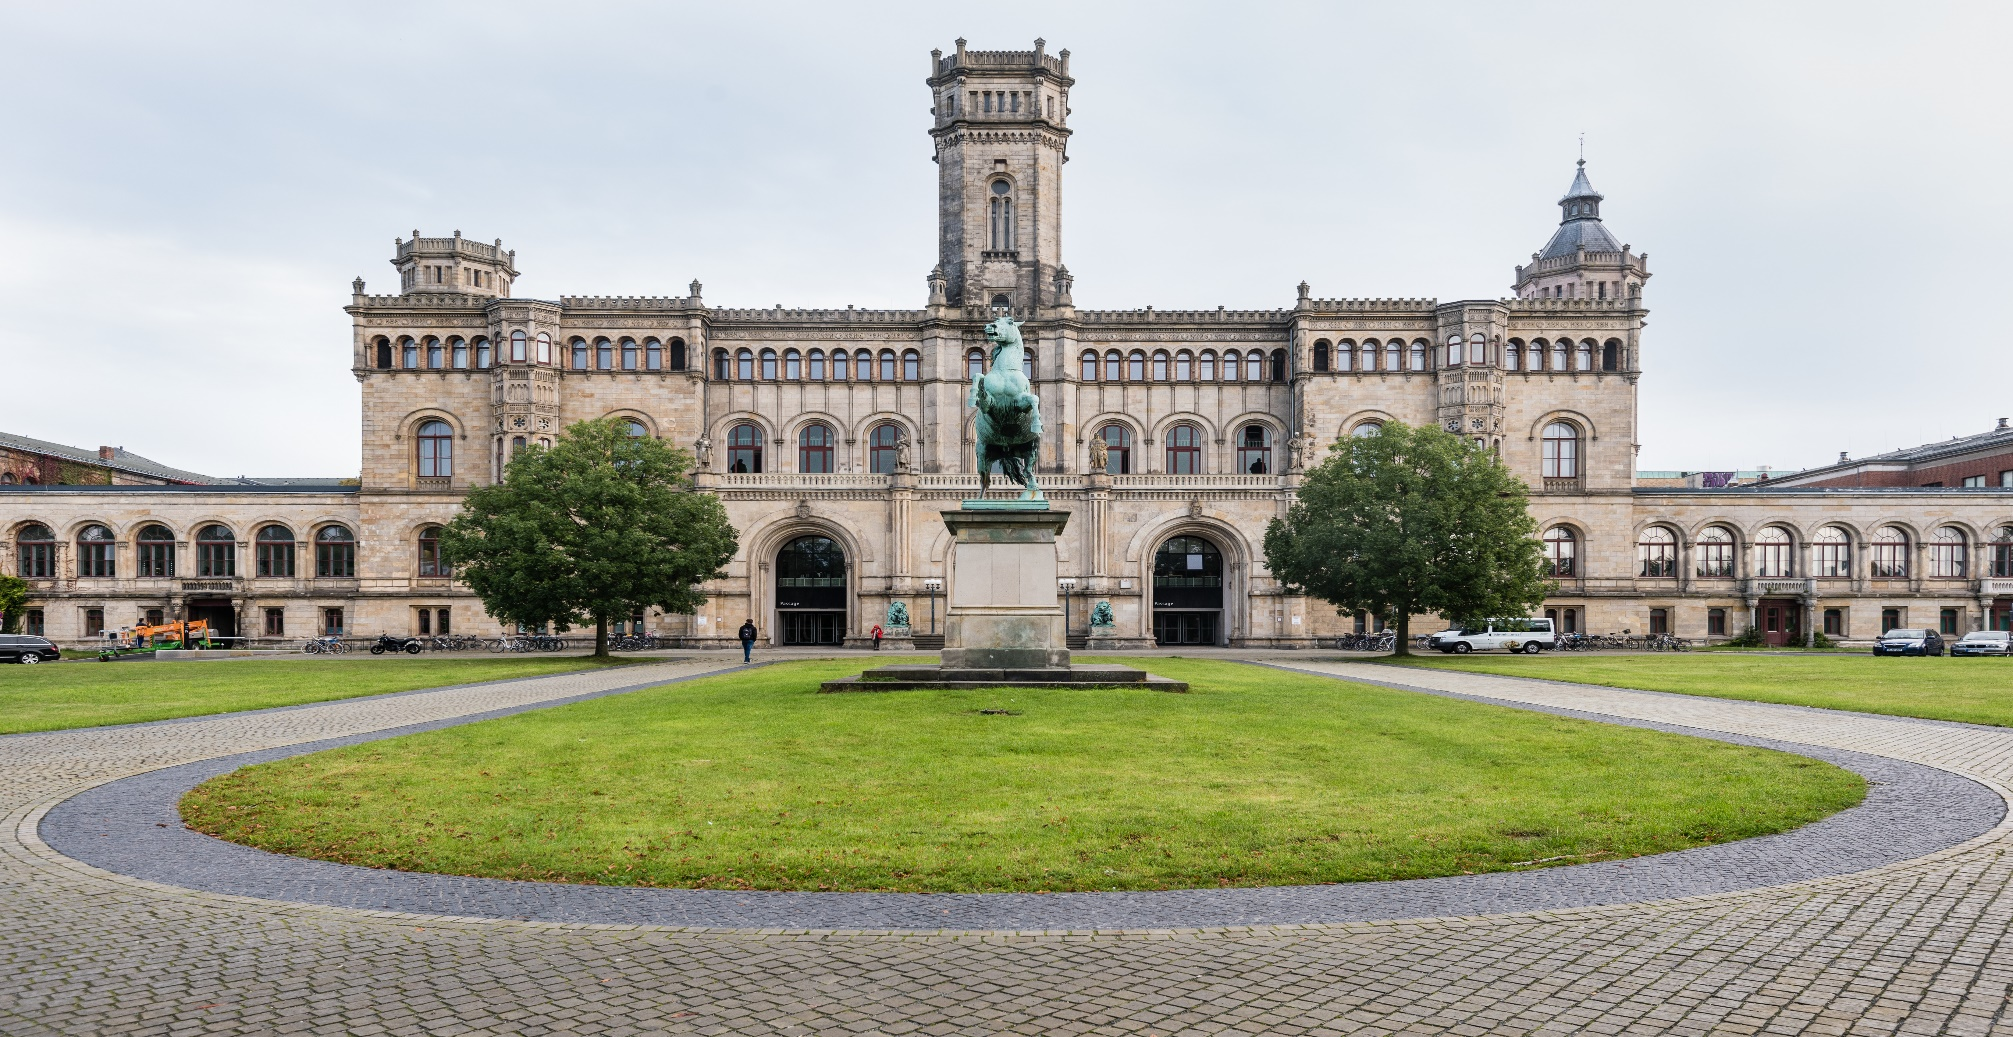
\includegraphics[width=.7\paperwidth]{img/welfenschloss.jpg}}

\newcommand{\footauthorcite}[1]{%
  \footnote{%
    \hangindent=2em % Adjust indentation for proper alignment
    \foreach \x in {#1} {%
        \citeauthor{\x} (\citeyear{\x}), \emph{\citetitle{\x}};
    }
  }%
}

\begin{document}

\begin{frame}
  \titlepage
\end{frame}

\begin{frame}{Table of Contents}
  \tableofcontents
\end{frame}

\AtBeginSection[]
{
  \begin{frame}{Table of Contents}
    \tableofcontents[currentsection]
  \end{frame}
}

%%%%%%%%%%%%%%%%%%%%%%%%%%%%%%%%%%%%%%%%%%
\section{Motivation}
\begin{frame}{Interpretable Style Embeddings}
  \begin{itemize}
    \item
  \end{itemize}
\end{frame}

\begin{frame}{Group-Specific Explanations}
  \begin{itemize}
    \item
  \end{itemize}
\end{frame}


%%%%%%%%%%%%%%%%%%%%%%%%%%%%%%%%%%%%%%%%%%
\section{Data Collection}
\begin{frame}{Group-Specific Texts}

\end{frame}


%%%%%%%%%%%%%%%%%%%%%%%%%%%%%%%%%%%%%%%%%%
% or Creation of the synthetic dataset?
\section{Creation of the Style Vector Attributes}
\subsection{Style Sentence Generation}
\begin{frame}{}

\end{frame}

\subsection{Clustering and Cluster Selection}
\begin{frame}{}

\end{frame}


%%%%%%%%%%%%%%%%%%%%%%%%%%%%%%%%%%%%%%%%%%
\section{Custom Models}
\subsection{SFAM}

\subsection{LISA}

\subsection{Embedding Model}


%%%%%%%%%%%%%%%%%%%%%%%%%%%%%%%%%%%%%%%%%%
\section{Steering Text Generation}
\subsection{Steering with Prompt Engineering}

\subsection{Activation Steering}


%%%%%%%%%%%%%%%%%%%%%%%%%%%%%%%%%%%%%%%%%%
\section{Conclusion}



%%%%%%%%%%%%%%%%%%%%[%%%%%%%%%%%%%%%%%%%%%%
\begin{frame}[c]
  \centering \Large
  Thank you for your attention
\end{frame}


\section*{References}
\begin{frame}[allowframebreaks]{References}
  \printbibliography
\end{frame}


\end{document}
